\section{Neural Architecture Search (NAS)} \label{section:nas}
 \glsreset{NAS}
Most neural architectures are created by specialists, which is labour-intensive and susceptible to other weaknesses, including the need for an extensive expertise and the potential to introduce human bias. Subsequently, a way of automatically designing and developing such algorithms has been a research field for a couple of years. \gls{NAS} aims to automate the previously manual process of designing architectures \autocite{elsken2019neural}. Consequently, \gls{NAS} is a sub-field of \gls{AutoML}. 

Given a search space $F$, a training set $D_{\text{train}}$, validation set $D_{\text{valid}}$ and an evaluation metric $M$, a \gls{NAS} algorithm aims at finding an optimal architecture $f^* \in F$ with the best metric $M^*$ (such as validation accuracy) on the validation set $D_{\text{valid}}$. This can be written mathematically as shown in \cref{eq:nas}

\begin{equation}\label{eq:nas}
\begin{aligned}
    f^* &= \text{argmax}_{f \in F} M(f(\theta^*), D_{\text{valid}}), \\
    \theta^* &= \text{argmin}_{\theta} L(f(\theta), D_{\text{train}}),
\end{aligned}
\end{equation}

where $\theta^*$ is the learned parameters for the architecture $f$ and $L$ is the loss function \autocite{zhou2019auto}. 

\Cref{fig:nas_overview} illustrates the overall concept of \gls{NAS}. The search space gives the algorithm constraints regarding its development by defining a set of architectural choices the model might use. For example, a constraint might be different operations such as convolution, fully connected and pooling. One might argue that this is vital as selecting the search space can reduce the search's complexity, which is essential to produce an acceptable model \autocite{kyriakides2020introduction}.


\begin{figure}[h]
\begin{tikzpicture}
    \node (space) [rectangle, minimum width=3cm, minimum height=1.5cm, text centered, draw=black, align=center] {Search Space \\ $\mathcal{A}$};
    \node (strategy) [rectangle, minimum width=3cm, minimum height=1.5cm, text centered, draw=black, right=of space, xshift=1cm] {Search Strategy};
    \node (performance) [rectangle, minimum width=3cm, minimum height=1.5cm, text centered, draw=black, right=of strategy, xshift=1cm, align=center] {Performance\\ Estimation\\ Strategy};

    \draw[->, >=stealth, bend left] (strategy) to node[midway, above, align=center] {architecture \\ $A \in \mathcal{A}$} (performance);
    \draw[->, >=stealth, bend left] (performance) to node[midway, below, align=center] {performance \\ estimation of $A$} (strategy);

    \draw[thick, ->, >=stealth] (space) --(strategy);
\end{tikzpicture}
    \caption{An overview of the different methods in NAS \autocite{elsken2019neural} }
    \label{fig:nas_overview}
\end{figure}

After defining a search space for the given problem, the search strategy will specify how to analyse the search space and propose a set of candidate architectures. This introduces the exploration-exploitation trade-off, which indicates that selecting an appropriate optimisation technique is vital because we want to find a global optimum and ensure that the search space is sufficiently investigated \autocite{kyriakides2020introduction}. 

The framework must perform performance estimation for each candidate architecture to adjust the search strategy. The simplest solution is to train and validate the model. However, this might require many hours of training, which requires a lot of energy and has a high environmental cost. Another downside of training the architectures is that it will limit the number of architectures the search algorithm might discover. As a result, methods simplifying this phase have been undergoing heavy research \autocite{elsken2019neural}. 

Ultimately, the goal of NAS is to automatically discover the most optimal architecture regarding performance and processing power. 

\subsection{Challenges}
\subsubsection{Computational power}
The most straightforward approach to determine the performance of a neural network is to train it until the validation accuracy has converged against a value or has been run for a fixed amount of epochs. However, training thousands of architectures may require hundreds or more GPU days \autocite{ren2021comprehensive}. The computational power required may be available for larger companies with plentiful resources. However, for most users, this is computationally infeasible. As a result, the necessary computational power is considered a significant challenge for NAS. 

\subsubsection{Black-box optimisation and lack of interpretability}
NAS algorithms often treat the architecture search space as a black box, meaning they cannot access the internal workings of the searched model architectures. This can make it difficult to incorporate domain knowledge or bias the search towards certain types of architectures. This results in difficult-to-interpret architectures, making it challenging to understand how they make predictions or identify potential problems with the architecture. \autocite{https://doi.org/10.48550/arxiv.1806.09055}

\subsection{Search Space}
When searching for a high-performing architecture, there are infinite variations that one might investigate. As a result, one defines a search space that gives the search algorithm constraints regarding what kind of combinations it might examine. Prior knowledge of what kind of search space is effective on specific tasks may reduce the size, but it has the disadvantage of introducing human bias in the search space \autocite{elsken2019neural}.  

Global search space is a way in which it tries to combine all possible operations to create chain-structured (sequential) networks. Then, the search space has the following parameters:
\begin{itemize}
    \item the number of layers
    \item the type of each operation
    \item the hyperparameters of each operation, namely kernel size, number of filters etc. 
\end{itemize}

Such a network can be described as a sequence of $n$ layers, where layer $L_i$ takes $L_{i-1}$ as input. However, this sort of search space is enormous and very expensive. 

Cell-based representations were inspired by successful architectures using repeated modules (Inception, ResNet). NASNet paper \autocite{DBLP:journals/corr/ZophVSL17}, is one of the most popular cell- or block-based approaches. Cell-based representations differ from global search space because they search for cells or blocks instead of whole architectures \autocite{elsken2019neural}. \cite{DBLP:journals/corr/ZophVSL17} learns two sorts of cells; a normal cell which performs feature extraction (preserving dimensionality), and a reduction cell which reduces the dimensionality. By stacking such cells, we get the final architecture, as shown in \cref{fig:cells}. 

\clearpage

\begin{figure}
    \centering
    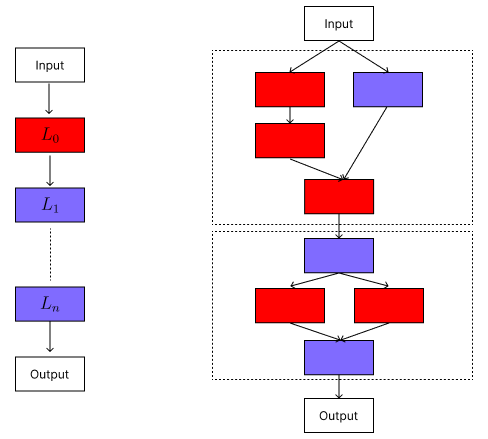
\includegraphics[width=8cm]{figures/cells.png}
    \caption{Left: chain-structured network, right: cells combined into an architecture}
    \label{fig:cells}
\end{figure}

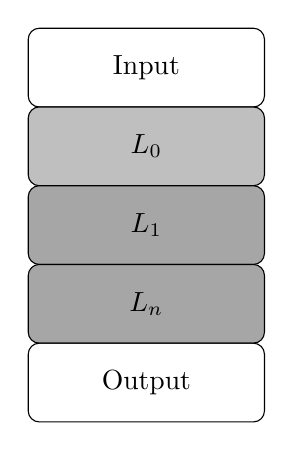
\begin{tikzpicture}
    \node (input) [rectangle, rounded corners, text centered, draw=black, minimum width=3cm, minimum height=1cm] {Input};
    \node (l0) [rectangle, rounded corners, text centered, draw=black, fill=gray!50, minimum width=3cm, minimum height=1cm, below of=input] {$L_0$};
    \node (l1) [rectangle, rounded corners, text centered, draw=black, fill=gray!70, minimum width=3cm, minimum height=1cm, below of=l0] {$L_1$};
    \node (ln) [rectangle, rounded corners, text centered, draw=black, fill=gray!70, minimum width=3cm, minimum height=1cm, below of=l1] {$L_n$};
    \node (output) [rectangle, rounded corners, text centered, draw=black, minimum width=3cm, minimum height=1cm, below of=ln] {Output};
\end{tikzpicture}

\clearpage

\subsubsection{Directed Acyclic Graphs}
\glsreset{DAG}
\Gls{DAG} is often used in \gls{NAS} to represent the structure of a neural network. In this context, the graph's vertices represent different operations or layers in the network, and the graph's edges represent the data flow between these operations. This allows researchers to efficiently represent and manipulate the structure of a neural network during the search process.

One of the main advantages of using \glspl{DAG} in \gls{NAS} is that they provide a convenient way to encode the constraints on the network architecture. For example, a \gls{DAG} can enforce the requirement that a neural network must have a certain number of layers or that individual layers must be connected in a specific way. This can help ensure that the search process only considers valid network architectures, which can speed up the search and improve its accuracy \autocite{https://doi.org/10.48550/arxiv.1806.09055}. 

In addition to representing the structure of a neural network, \glspl{DAG} can also represent the search space over which the architecture search algorithm operates. This allows the algorithm to explore different network architectures efficiently and evaluate their performance, ultimately discovering novel and effective network architectures \autocite{inproceedings}. 

\subsection{Search Strategies}

\subsubsection{Random Search}
Random search is the most naive search strategy, and it will simply randomly pick a good architecture based on the search space. Therefore, the method is relatively fast and does not require any learning model. A random search may be effective if a search space is well constructed.  

\subsubsection{Reinforcement Learning}
On the very basic, reinforcement learning is an area within machine learning in which an agent learns behaviour by some trial-and-error interaction with a dynamic environment \autocite{kaelbling1996reinforcement}. One can consider \gls{NAS} a reinforcement problem by looking at the creation of the architecture as the agent's action, in which the action space is the problem's search space. The agent gets rewarded depending on the performance of the trained architecture. There are numerous approaches to representing an agent's policy, such as a recurrent neural network, proximal policy optimisation and q-learning \autocite{elsken2019neural}. 

\subsubsection{Evolutionary algorithms}
Evolutionary algorithms are techniques used in optimisation and search methods. It is a subset of \gls{EC} and is an effective way of problem-solving for often encountered global optimisation problems because of its adaptable character \autocite{7955308}. Evolutionary algorithms in \gls{NAS} randomly select $N$ initialised models and then assess performance by the given evaluation strategy. The best models are chosen as parents, and new models have mutated clones of the parents, which are re-evaluated. Finally, the worst $N$ models are removed from the population to make room for new offspring \autocite{https://doi.org/10.48550/arxiv.1703.01041}. 

\subsubsection{Bayesian optimisation}
\Gls{BO} has been a popular approach for hyperparameter optimisation \autocite{elsken2019neural}. In general, \gls{BO} optimises expensive functions to evaluate, such as the performance of architectures. This is a global optimisation problem that \gls{BO} tries to solve. Given a costly to evaluate function $f$, \gls{BO} aims at finding its optimal score within some domain $x$ \autocite{kandasamy2018neural}. In other words, \gls{BO} pursues to calculate $a^* = arg min_{a \in A} f(a)$, where A is the given search space, and $f(a)$ is the performance function of the neural network after training the architecture $a$ for a fixed number of iterations \autocite{white2021bananas}.  

\subsection{Performance Estimation}
\subsubsection{Performance Predictors}\label{sec:performancepredictors}
As mentioned in \cref{section:nas}, \gls{NAS} aims to automate the process of designing high-performing neural networks. However, this often requires training all the candidate networks, either partly or wholly, to get the accuracy of the neural networks. In most cases, this is an infeasible approach when the search space is big, which is why performance predictors are introduced \autocite{akhauri2022evolving}. 

Any function that forecasts the eventual accuracy or ranking of architectures without fully training the architecture is referred to as a performance predictor $f$. Therefore, the performance predictor's function should take significantly less time than training and validating the neural network fully and have a high correlation or rank correlation with the validation error \autocite{white2021powerful}. 

A performance predictor is defined by two main routines - initialisation and query. The initialisation routine does some general pre-computation, often before the \gls{NAS} algorithm. For model-based methods, the initialisation routine consists of fully training a set of architectures to get data points. Then, the query routine will output the predicted accuracy with the architecture details as input \autocite{white2021powerful}. 

There exist multiple categories of performance predictors:

\begin{table}[h]
\caption{List of performance predictors}
\centering
\begin{tabular}{|l}
Model-based (trainable) methods \\
\cellcolor{verylightgray}Learning curve-based methods    \\
Hybrid methods                  \\
\cellcolor{verylightgray}Zero-cost proxies               \\
Weight sharing methods         
\end{tabular}
\end{table}

\subsubsection{Zero-Cost Proxies}\label{subsec:zerocost}
Zero-cost proxies are a class of performance predictors. The name zero-cost comes from analysing a neural network at initialisation, indicating that it costs 'zero' to generate the score. At the same time, the predicted accuracy is closely correlated with the actual accuracy. 

By performing a single forward/backward propagation pass using a single minibatch of data, zero-cost proxies methods can score a neural network \autocite{akhauri2022evolving}. The intuition is that one can measure the 'trainability' of a neural network by looking at the initial gradient flow. 

The paper \textit{Zero-Cost Proxies for Lightweight NAS}, \autocite{abdelfattah2021zero} showed the usefulness of a range of zero-cost proxies inspired by the pruning-at-initialisation literature. Each method can be divided into two categories - data-independent or data-dependent. 

Data-dependent zero-cost proxies use data to generate the score, whereas data-independent will not use the dataset in principle. Sometimes, it is used to set dimensions \autocite{colin2022adeeperlook}. \Cref{tab:zcproxies} lists data-independent and data-dependent zero-cost proxies. However, this collection is not exhaustive, and additional zero-cost proxies are not included. 


\begin{table}[ht]
    \caption{Different zero-cost proxies within the two categories data-independent and data-dependent}
    \centering
    \begin{tabular}{l|l}
    \textbf{Data-independent}         & \textbf{Data-dependent} \\ \hline
    Synflow & EPE-NAS                   \\
    \cellcolor{verylightgray}Zen-score                       & \cellcolor{verylightgray}Fisher                    \\
    GenNAS                          & Grad-norm                 \\
    \cellcolor{verylightgray}number of parameters in network & \cellcolor{verylightgray}Grasp                                 
    \end{tabular}
    \label{tab:zcproxies}
\end{table}


